% Chapter 2

\chapter{Dynamic programming in Bioinformatics} % Main chapter title

\label{DynamicProg} % For referencing the chapter elsewhere, use \ref{Chapter1} 

\lhead{Chapter 2. \emph{Dynamic programming in Bioinformatics}} % This is for the header on each page - perhaps a shortened title

Dynamic Programming (DP) \citep{BioMach} is a optimization technique that recursively breaks down a problem into smaller subproblems, such that the solution to the larger problem can be obtained by piecing together the solutions to the subproblems. This section shows how the Smith-Waterman algorithms and the algorithms in HMMER use DP for sequence alignment and database searches.

%----------------------------------------------------------------------------------------

\section{The Smith-Waterman algorithm}


%----------------------------------------------------------------------------------------

\section{HMMER}

\label{HMMERsect}

HMMER \citep{HMMER} is a set of applications that create a profile Hidden Markov Model (HMM) of a sequence family which can be utilized as a query against a sequence database to identify (and/or align) additional homologs of the sequence family\citep{Seq}. HMMER was developed by Sean Eddy at Washington University and has become one of the most widely used software tools for sequence homology. The main elements of this HMM-based sequence alignment package are \emph{hmmsearch} and \emph{hmmscan}. The former searches for a profile HMM in a sequence database, while the latter searches for one or more sequences in profile HMMs database.

\subsection{HMM and profile HMM}

A hidden Markov model (HMM) is a computational structure for linearly analyzing sequences with a probabilistic method\citep{DicBioinfo}. HMMs have been widely used in speech signal, handwriting and gesture detection problems. In bioinformatics they have been used for applications such as sequence alignment, prediction of protein structure, analysis of chromosomal copy number changes, and gene-finding algorithm, etc\citep{BioFunc}. 

A HMM is a type of a non-deterministic finite state machine with transiting to another state and emitting a symbol under a probabilistic model.
According to \citep{SeqData}, a HMM can be defined as a 6-tuple ($A$, $Q$, $q_0$, $q_e$, $tr$, $e$) where \\[-1cm]

\begin{itemize}
\item \textbf{$A$} is a finite set (the alphabet) of symbols;
\item \textbf{$Q$} is a finite set of \emph{states};
\item \textbf{$q_0$} is the \emph{start} state and \textbf{$q_e$} is the \emph{end} state;
\item \textbf{$tr$} is the \emph{transition} mapping, which is the transition probabilities of state pairs in $Q$ $\times$ $Q$, satisfying the following two conditions: 
  \begin{enumerate}
   \item[(a)] $0 \leqslant tr(q,q') \leqslant 1$, $\forall q,q' \in Q$, and
   \item[(b)] for any given state $q$, such that:
   \begin{equation*}
    \displaystyle\sum_{q' \in Q}tr(q,q') = 1
   \end{equation*}
  \end{enumerate}
\item \textbf{$e$} is the \emph{emission} mapping, which is the emission probabilities of pairs in $Q$ $\times$ $A$, satisfying the following two conditions:
  \begin{enumerate}
   \item[(a)] $0 \leqslant e(q,x) \leqslant 1$, if it is defined, $\forall q \in Q$, and $x \in A$
   \item[(b)] for any given state $q$, if for any $x \in A$, $e(q, x)$ is defined, then $q$ is an \emph{emitting} state and
   \begin{equation*}
    \displaystyle\sum_{x \in A}e(q,x) = 1 
   \end{equation*}
   if $\forall x \in A$, $e(q, x)$ is not defined, then $q$ is a \emph{silent} state.
  \end{enumerate}
\end{itemize}

The dynamics of the system is based on Markov Chain, meaning that only the current state influences the selection of its successor – the system has no 'memory' of its history. Only the succession of characters emitted is visible; the state sequence that generated the characters remains internal to the system, i.e. hidden. By this means, the name is Hidden Markov Model\citep{IntroBio}. 

Profile HMM is a variant of HMM and can be constructed from an initial multiple sequence alignment to define a set of probabilities. The symbol sequence of an HMM is an observed sequence that resembles a consensus for the multiple sequence alignment. And a protein or gen family can be defined by profile HMMs.

In Figure\ref{fig:pHMM}, the internal structure of the "Plan 7" profile HMM used by HMMER\citep{HMMER3} shows the mechanism for generating sequences. In order to generate sequences, a profile HMM should have a set of three states per alignment column: one \emph{match} state, one \emph{insertion} state and one \emph{deletion} state. 
\begin{itemize}
\item \textbf{\emph{Match states}} match and emit a amino acid from the query. The probability of emitting each of the 20 amino acids is a property of the model. 
\item \textbf{\emph{Insertion states}} allows the insertion of one or more amino acids. The emission probability of this state is computed either from a background distribution of amino acids or from the observed insertions in the alignment.
\item \textbf{\emph{Deletion states}} skip the alignment column and emit a blank. Entering this state corresponds to gap opening, and the probabilities of these transitions reflect a position-specific gap penalty.
\end{itemize}

\begin{figure}[!htb]
	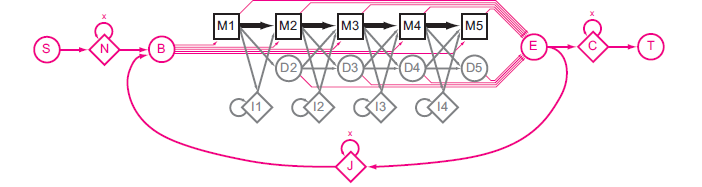
\includegraphics[width=150mm]{Figures/pHMM.png}
	\caption{Profile HMM architecture used by HMMER\citep{HMMER3}.}
	\label{fig:pHMM}
\end{figure}

Begin at Start(S), and follow some chain of arrows until arriving at Termination(T). Each arrow transits to a state of the system. 
At each state, an action can be taken either as (1) emitting a residue\footnote{In this thesis, \emph{residue} is used to refer to amino acids for protein or to nucleotides for DNA/RNA.}, or (2) selecting an arrow to the next state. The action and the selection of successor state are governed by sets of probabilities\citep{IntroBio}.
The linear core model has five sets of match (M), insertion (I) and deletion (D) states. Each M state represents one consensus position and a set of M, I, D states is the main element of the model and is referred to as a “node” in HMMER. Additional flanking states (marked as N, C, and J) emit zero or more residues from the background distribution, modelling nonhomologous regions preceding, following, or joining homologous regions aligned to the core model. Start (S), begin (B), end (E) and termination (T) states are non-emitting states.


A profile HMM for a protein family can be used to compare with query sequences, and classify sequences that are members of the family and those which are not\citep{ProteinBio}. 
A common application of profile HMMs is used to search a profile HMM against a sequence database. Another application is the query of a single protein sequence of interest against a database of profile HMMs.

\subsection{Viterbi algorithm in HMMER2}

\label{ViterbiSub}

In HMMER2, both \emph{hmmsearch} and \emph{hmmpfam} rely on the same core Viterbi algorithm for their scoring function which is named as \emph{P7Viterbi} in codes.

To find whether a sequence is member of the family described by a HMM, we compare the sequence with the HMM. We use an algorithm known as Viterbi to find one path that has the maximum probability of the HMM generating the sequence. Viterbi is a dynamic programming algorithm. Let $V_{i,j}$ be the maximum probability of a path from the start state $S_i$ ending at state $S_j$ and generating the prefix $q_{1...j}$ of the query. $V_{i+1,j}$ is found by the recurrence:

\begin{equation*}
   \displaystyle V_{i+1,j} = \max_{0 \leqslant k \leqslant j-1} \big ( V_{i,k} P(k,j)P(q_{i+1} |j) \big )
\end{equation*}

% max |x| = 
%     \begin{cases}
%     \quad -x & \text{if } x < 0,\\
%     0 & \text{if } x = 0,\\
%     x & \text{if } x > 0.
%     \end{cases}
%     max = \left\{
% \begin{array}{rl}
% -x & \text{if } x < 0,\\
% 0 & \text{if } x = 0,\\
% x & \text{if } x > 0.
% \end{array} \right.

Define $a_{ij}$ as the transition probability from state $i$ to $j$ and $e_i$ as emission probability in state $i$.
Define $V_j^M(i)$ as the log-odds score of the optimal path matching subsequence $x_{1...i}$ to the submodel up to state $j$, ending with $x_i$ being emitted by \emph{match} state $M_j$. Similarly $V_j^I(i)$ is the score of the optimal path ending in $x_i$ being emitted by \emph{insertion} state $I_j$, and $V_j^D(i)$ for the optimal path ending in \emph{deletion} state $D_j$. $q_{x_i}$ is the probability of $x_i$. Then we can write the Viterbi general equation\citep{BioSeq}:

\begin{equation*}
   V_j^M(i) = \log\frac{e_{M_j}(x_i)}{q_{x_i}} + max 
   \begin{cases}
   V_{j-1}^M(i-1) + \log a_{M_{j-1}M_j}\\
   V_{j-1}^I(i-1) + \log a_{I_{j-1}M_j}\\
   V_{j-1}^D(i-1) + \log a_{D_{j-1}M_j}
   \end{cases}
\end{equation*}

\begin{equation*}
   V_j^I(i) = \log\frac{e_{I_j}(x_i)}{q_{x_i}} + max 
   \begin{cases}
   V_j^M(i-1) + \log {a}_{M_jI_j}\\
   V_j^I(i-1) + \log a_{I_jI_j}
   \end{cases} 
\end{equation*}

\begin{equation*}
   V_j^D(i) = max 
   \begin{cases}
   V_{j-1}^M(i) + \log a_{M_{j-1}D_j}\\
   V_{j-1}^D(i) + \log a_{D_{j-1}D_j}
   \end{cases}  
\end{equation*}

The efficient DP-based pseudo code of Viterbi algorithm is shown in Algorithm\ref{Viterbi} \citep{FPGA}.  The inner loop of the code contains three two dimensional matrices (M, I, D), which calculate scores of all node positions involved in the main models for each of the residue. The outer loop consists of flanking and special states calculated in the one dimensional arrays N, B, C, J, E .

\renewcommand{\thepseudonum}{\roman{pseudonum}}
\begin{pseudocode}{Viterbi}{ }
\label{Viterbi}
\COMMENT{Initialization}\\
N[0] \GETS 0; \ \  B[0] \GETS tr(N, B)\\
E[0] \GETS C[0] \GETS J[0] \GETS -\infty\\
\COMMENT{for every sequence residue i}\\
\FOR i \GETS 1 \TO n \DO
\BEGIN
  N[i] \GETS N[i-1] + tr(N, N)\\
  B[i] \GETS max 
  \begin{cases}
   N[i-1] + tr(N, B)\\
   J[i-1] + tr(J, B)
  \end{cases}\\
  M[i,0] \GETS I[i,0] \GETS D[i,0] \GETS -\infty\\
  \COMMENT{For every model position j from 1 to m}\\
  \FOR j \GETS 1 \TO m \DO
  \BEGIN
    M[0, j] \GETS I[0, j] \GETS D[0, j] \GETS -\infty\\
    M[i, j] \GETS e(M_j, S[i]) + max 
    \begin{cases}
     M[i-1, j-1] + tr(M_{j-1}, M_j)\\
     I[i-1, j-1] + tr(I_{j-1}, M_j)\\
     D[i-1, j-1] + tr(D_{j-1}, M_j)\\
     B[i-1] + tr(B, M_j)
    \end{cases}\\
    I[i, j] \GETS e(I_j, S[i]) + max
    \begin{cases}
     M[i-1, j] + tr(M_j, I_j)\\
     I[i-1, j] + tr(I_j, I_j)
    \end{cases}\\
    D[i, j] \GETS max
    \begin{cases}
     M[i, j-1] + tr(M_{j-1}, D_j)\\
     D[i, j-1] + tr(D_{j-1}, D_j)
    \end{cases}\\
  \END\\
  E[i] \GETS max\{M[i,j] + tr(M_j, E)\} \ \  (j \GETS 0 \TO m-1)\\
  J[i] \GETS max 
  \begin{cases}
   J[i-1] + tr(J, J)\\
   E[i-1] + tr(E, J)
  \end{cases}\\
  C[i] \GETS max
  \begin{cases}
   C[i-1] + tr(C, C)\\
   E[i-1] + tr(E, C)
  \end{cases}\\
\END\\
\COMMENT{Termination: }\\
\RETURN {T(S,M) \GETS C[n] + tr(C,T)}
\end{pseudocode}

\subsection{MSV algorithm in HMMER3}

\label{MSVsub}

HMMER3 is near rewrite of the earlier HMMER2 package, with the aim of improving the speed of profile HMM searches. The main performance gain is due to a heuristic algorithm called MSV filter, for Multiple (local, ungapped) Segment Viterbi. MSV is implemented in SIMD(Single-Instruction Multiple-Data) vector parallelization instructions and is about 100-fold faster than HMMER2.

\begin{figure}[!htb]
	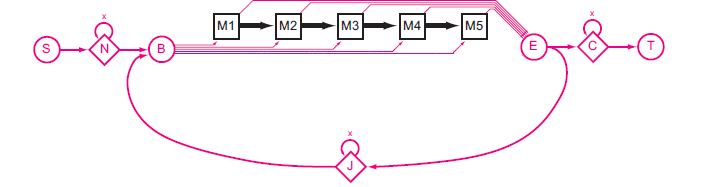
\includegraphics[width=150mm]{Figures/pHMM_msv.png}
	\caption{MSV profile: multiple ungapped local alignment segments\citep{HMMER3}.}
	\label{fig:pMSV}
\end{figure}

Figure\ref{fig:pMSV} illustrates the MSV profile architecture. Compared with Figure\ref{fig:pHMM}, the MSV corresponds to the virtual removal of the deletion and insertion states. All match-match transition probabilities are treated as 1.0. The rest parameters remains unchanged. So this model generates sequences containing one or
 more ungapped local alignment segments. The pseudo code of MSV score algorithm is simplified and shown in Algorithm\ref{MSV}.

\begin{pseudocode}{MSV}{ }
\label{MSV}
\COMMENT{Initialization}\\
N[0] \GETS 0; \ \  B[0] \GETS tr(N, B)\\
E[0] \GETS C[0] \GETS J[0] \GETS -\infty\\
\COMMENT{for every sequence residue i}\\
\FOR i \GETS 1 \TO n \DO
\BEGIN
  N[i] \GETS N[i-1] + tr(N, N)\\
  B[i] \GETS max 
  \begin{cases}
   N[i-1] + tr(N, B)\\
   J[i-1] + tr(J, B)
  \end{cases}\\
  M[i,0] \GETS -\infty\\
  \COMMENT{For every model position j from 1 to m}\\
  \FOR j \GETS 1 \TO m \DO
  \BEGIN
    M[0, j] \GETS -\infty\\
    M[i, j] \GETS e(M_j, S[i]) + max 
    \begin{cases}
     M[i-1, j-1]\\
     B[i-1] + tr(B, M_j)
    \end{cases}\\
  \END\\
  E[i] \GETS max\{M[i,j] + tr(M_j, E)\} \ \  (j \GETS 0 \TO m-1)\\
  J[i] \GETS max 
  \begin{cases}
   J[i-1] + tr(J, J)\\
   E[i-1] + tr(E, J)
  \end{cases}\\
  C[i] \GETS max
  \begin{cases}
   C[i-1] + tr(C, C)\\
   E[i-1] + tr(E, C)
  \end{cases}\\
\END\\
\COMMENT{Termination: }\\
\RETURN {T(S,M) \GETS C[n] + tr(C,T)}
\end{pseudocode}

\subsubsection*{SIMD vector parallelization in HMMER3}
\label{SSE2}

Single-Instruction Multiple-Data (SIMD) instruction is able to perform the same operation on multiple pieces of data in parallel. The SIMD vector instruction sets use 128-bit vector registers to compute up to 16 simultaneous operations. Several SIMD vector parallelization methods have been described for accelerating Smith-waterman dynamic programming. Rognes and Seeberg \citep{SW-SIMD} presented an implementation of the Smith–Waterman algorithm running on the Intel Pentium processor using the MMX SIMD instructions. A six-fold speedup was reported over an optimized non-SIMD implementation. Farrar \citep{SW-SSE2} presented an efficient vector-parallel approach called striped Smith-Waterman using Intel Streaming SIMD Extensions 2 (SSE2). A speedup of 2–8 times was reported over the Rognes and Seeberg SIMD implementations.

Similarly, since the MSV model removes deletion and insertion states that interfere with vector parallelism, the striped vector-parallel technique can be remarkably efficient way to calculate MSV alignment scores. To maximize parallelism, in HMMER3\citep{HMMER3}, Sean R. Eddy implemented MSV as a 16-fold parallel calculation with score values stored as 8-bit byte integers. He used SSE2 instructions on Intel-compatible systems and Altivec/VMX instructions on PowerPC systems.

Figure\ref{fig:strip} shows the stripped pattern. The query profile HMM of length $m$ is divided into vectors with equal length $v$. The vector length $v$ is equal to the number of elements being processed in the 128-bit SIMD register. MSV processes 8-bit byte integer with $v$ = 128/8 = 16. In a row-vectorized implementation, the query profile HMM is stored in the vectorized dynamic programming matrix dp. dp stores $m$ cells in $Q$ vectors which is numbered as $q = 1...Q$, where $Q = (m+v-1)/v$. Figure\ref{fig:strip} illustrates $m$ cells assigned to $Q$ vectors in a non-sequential way. For simple illustration, $v = 4, m = 14$, and $Q = 4$.

\begin{figure}[!htb]
	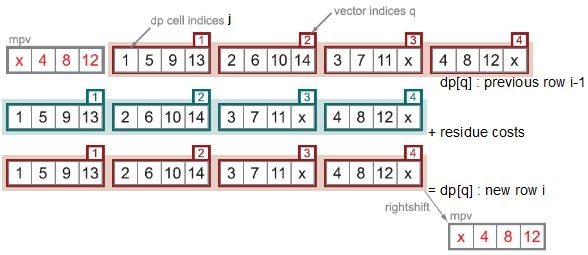
\includegraphics{Figures/msv_vector.jpg}
	\caption{Illustration of striped indexing for SIMD vector calculations\citep{HMMER3}.}
	\label{fig:strip}
\end{figure}

In Smith-Waterman and Viterbi dynamic programming, the calculation of each cell $(i, j)$ in the dp is dependent on previously calculated cells $(i-1, j), (i, j-1)$ and $(i-1, j-1)$. However, in MSV algorithm, the deletion and insertion states have been removed and only ungapped diagonals need calculating, so the calculation of each cell $(i, j)$ requires only previous $(i-1, j-1)$. In Figure\ref{fig:strip}, the top red row shows the previous row $i-1$ for the cells $j-1$, which is needed for calculating each new cell $j$ in a new row $i$. 

Striping method can remove the SIMD register data dependencies. As can be seen in the Figure\ref{fig:strip}, with striped indexing, vector $q-1$ contains exactly the four $j-1$ cells needed to calculate the four cells $j$ in a new vector $q$ on a new blue row of the dp matrix. For example, when we calculate cells $j=(2,6,10,14)$ in vector $q=2$, we access the previous row’s vector $q-1=1$ which contains the cells we need in the order we need them, $j-1=(1,5,9,13)$ (the vector above). 

\begin{figure}[!htb]
\centering
	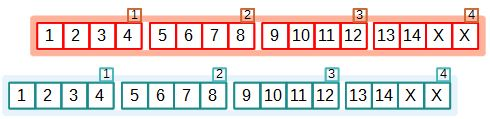
\includegraphics{Figures/msv_nostrip.jpg}
	\caption{Illustration of linear indexing for SIMD vector calculations.}
	\label{fig:nostrip}
\end{figure}

Instead, if we indexed cells into vectors in the linear order ($j=1,2,3,4$ in vector $q=1$ and so on), as shown in Figure\ref{fig:nostrip}, there is no such correspondence of $(q,q-1)$ with four $(j-1,j)$, and each calculation of a new vector $q$ would require extra expensive operations, such as shifting or rearranging cell values inside the previous row's vectors. By using the striped query access, only one shift operation is needed per row as shown in \ref{fig:strip}. Outside the inner loop(for $q = 1$ to Q), the last vector on each finished row is right-shifted (mpv, in grey with red cell $j$ indices) and used to initialize the next row calculation.

The pseudo code for the implementation is shown in Algorithm\ref{MSV-SIMD}

\begin{pseudocode}{MSV-SIMD}{ }
\label{MSV-SIMD}
\COMMENT{Initialization}\\
xJ \GETS 0; \ \  dp[q] \GETS vec\_splat(0) \  (q \GETS 0 \TO Q-1)\\
xB \GETS base + tr(N, B)\\
xBv \GETS vec\_adds(xB, tr(B, M))\\
\COMMENT{for every sequence residue i}\\
\FOR i \GETS 1 \TO n \DO
\BEGIN
  xEv \GETS vec\_splat(0)\\
  mpv \GETS vec\_rightshift(dp[Q-1])\\
  \FOR q \GETS 0 \TO Q-1 \DO
  \BEGIN
    \COMMENT{temporary  storage of 1 current row value in progress}\\
    tmpv \GETS vec\_max(mpv, xBv)\\
    tmpv \GETS vec\_adds(tmpv, e(M_j, S[i]))\\
    xEv \GETS vec\_max(xEv, tmpv)\\
    mpv \GETS dp[q]\\
    dp[q] \GETS tmpv\\
  \END\\
  xE \GETS vec\_hmax(xEv)\\
  xJ \GETS max 
  \begin{cases}
   xJ\\
   xE + tr(E, J)
  \end{cases}\\
  xB \GETS max 
  \begin{cases}
   base\\
   xJ + tr(J, B)
  \end{cases}\\
\END\\
\COMMENT{Termination: }\\
\RETURN {T(S,M) \GETS xJ + tr(C,T)}
\end{pseudocode}

Five pseudocode vector instructions for operations on 8-bit integers are used in the pseudo code. Either scalars $x$ or vectors v containing 16 8-bit integer elements numbered $v[0]...v[15]$. Each of these operations are either available or easily constructed in Intel SSE2 intrinsics as shown in the following table.

% \begin{minipage}{\textwidth}
% \begin{center}
% \begin{tabular}{|c|c|c|}\hline
% \shortstack{\textbf{Pseudocode} \\ SSE2 code in C} & \textbf{Operation} & \textbf{Definition}\\\hline
% \shortstack{\textbf{v = vec\_splat(x)} \\ v = \_mm\_set1\_epi8(x)} & assignment & $v[z] = x$\\\hline
% \shortstack{\textbf{v = vec\_adds(v1, v2)} \\ v = \_mm\_adds\_epu8(v1, v2)} & saturated addition & $v[z] = min$
% $\begin{cases}
%   2^8-1\\
%   v1[z]+v2[z]
% \end{cases}$\\\hline
% \shortstack{\textbf{v1 = vec\_rightshift(v2)} \\ v1 = \_mm\_slli\_si128(v2, 1)} & right shift & \shortstack{$v1[z] = v2[z-1](z=16...1)$; \\ $v1[0]=0;$}\\\hline
% \shortstack{\textbf{v = vec\_max(v1, v2)} \\ v = \_mm\_max\_epu8(v1, v2)} & max & $v[z] = max(v1[z], v2[z])$\\\hline
% \shortstack{\textbf{x = vec\_hmax(v)} \\ -} & horizontal max & $x = max_zv[z]$\\\hline
% \end{tabular}
% \end{center}
% \end{minipage}


\begin{table}[H]
\centering
\begin{tabular}{|c|c|c|}\hline
\shortstack{\textbf{Pseudocode} \\ SSE2 intrinsic in C} & \textbf{Operation} & \textbf{Definition}\\\hline
\shortstack{\textbf{v = vec\_splat(x)} \\ v = \_mm\_set1\_epi8(x)} & assignment & $v[z] = x$\\\hline
\shortstack{\textbf{v = vec\_adds(v1, v2)} \\ v = \_mm\_adds\_epu8(v1, v2)} & saturated addition & $v[z] = min$
$\begin{cases}
  2^8-1\\
  v1[z]+v2[z]
\end{cases}$\\\hline
\shortstack{\textbf{v1 = vec\_rightshift(v2)} \\ v1 = \_mm\_slli\_si128(v2, 1)\tablefootnote[10]{Because x86 and x86-64 use little endian, this means using a left bit shift intrinsic \_mm\_slli\_si128 to do right shift.}} & right shift & \shortstack{$v1[z] = v2[z-1](z=15...1)$; \\ $v1[0]=0;$}\\\hline
\shortstack{\textbf{v = vec\_max(v1, v2)} \\ v = \_mm\_max\_epu8(v1, v2)} & max & $v[z] = max(v1[z], v2[z])$\\\hline
\shortstack{\textbf{x = vec\_hmax(v)} \\ -\tablefootnote[11]{No SSE2 intrinsic is corresponding to vec\_hmax. Shuffle intrinsic \_mm\_shuffle\_epi32 and \_mm\_max\_epu8 can be combined to implement vec\_hmax.}} & horizontal max & $x = max(v[z]),z=0...15$\\\hline
\end{tabular}
\caption{SSE2 intrinsics for pseudocode in Algorithm\ref{MSV-SIMD}\label{tab.SSE2}}
\end{table}



%----------------------------------------------------------------------------------------
